\subsection{SG90 -- Mikro Servo}
\label{subsec:sg90_micro_servo}

% ---------------------------------------------------------------------
\subsubsection{Identitas dan Fungsi}

\begin{wrapfigure}{r}{0.25\textwidth}% 'r' untuk posisi kanan, '0.25\textwidth' untuk lebar gambar
	\vspace{-20pt}
	\centering
	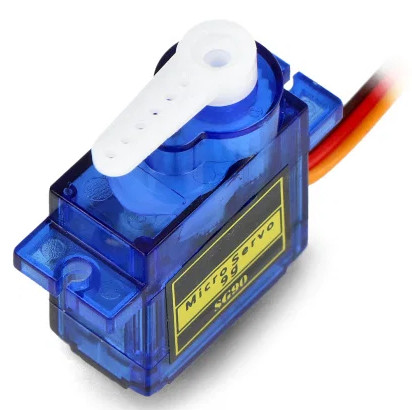
\includegraphics[width=\linewidth]{images/sg90-front.jpg} % Ganti dengan nama file gambar Anda
	\caption{Mikro servo SG90}
	\label{fig:sg90-front}
\end{wrapfigure}

SG90 adalah sebuah aktuator putar (\textit{rotary actuator}) berukuran mikro yang dirancang untuk mengendalikan posisi sudut mekanis secara presisi berbasis sistem \textit{feedback} tertutup (\textit{closed-loop control}). Komponen ini dikategorikan sebagai aktuator elektromekanis terintegrasi.

SG90 memiliki ukuran yang kompak, bobot yang sangat ringan ($\approx 9\,\text{g}$), harga yang terjangkau, serta antarmuka kontrolnya yang sederhana karena hanya membutuhkan satu jalur sinyal \textit{Pulse Width Modulation} (PWM) dari mikrokontroler tanpa memerlukan IC \textit{driver} tambahan.

\begin{table}[H]
	\centering
	\caption{Identitas komponen SG90 Mikro Servo}
	\label{tab:sg90_identitas}
	\small
	\begin{tabularx}{\textwidth}{@{} p{3.8cm} X @{}}
		\toprule
		Parameter          & Keterangan                                                                                     \\
		\midrule
		Nama komponen      & SG90 Micro Servo Motor                                                                         \\
		Model/part number  & SG90 / TowerPro SG90                                                                           \\
		Jenis              & Aktuator Elektromekanis / Servo Posisi Analog                                                  \\
		Fungsi utama       & Mengubah sinyal lebar pulsa PWM menjadi posisi sudut mekanis ($0^\circ \text{ s.d. } 180^\circ$) \\
		Sumber dokumentasi & TowerPro SG90 Micro Servo Motor Datasheet (FriendlyWire)                                       \\
		\bottomrule
	\end{tabularx}
\end{table}

% ---------------------------------------------------------------------
\subsubsection{Prinsip Kerja}
Cara kerja motor servo SG90 didasarkan pada sistem kendali umpan balik posisi tertutup (\textit{closed-loop position control}). Di dalam satu unit SG90, terdapat empat elemen utama yang bekerja bersama:

\begin{enumerate}
	\item \textbf{Bagian Penggerak dan Mekanis (Motor DC \& Rangkaian Roda Gigi):}
	      Sebuah motor DC kecil berputar dengan kecepatan tinggi ketika dialiri arus listrik. Putaran motor ini kemudian diteruskan ke rangkaian roda gigi nilon (\textit{gearbox}) untuk menurunkan kecepatan putar sekaligus meningkatkan torsi (daya dorong mekanis) pada poros luar (\textit{output horn}).

	\item \textbf{Bagian Penginderaan dan Pembanding Sinyal (Potensiometer \& IC Driver):}
	      Poros utama terhubung langsung secara mekanis ke sebuah potensiometer internal yang berfungsi sebagai pembaca posisi sudut aktual ($\theta_{\text{aktual}}$). IC pengendali internal secara kontinu membandingkan nilai tegangan dari potensiometer dengan lebar pulsa sinyal PWM yang diterima dari mikrokontroler:
	      \begin{itemize}
		      \item Jika posisi poros belum sesuai dengan sudut perintah, IC mengalirkan arus ke motor DC untuk memutar roda gigi ke arah target.
		      \item Ketika potensiometer mendeteksi bahwa poros telah mencapai sudut yang diinginkan, IC menghentikan pasokan arus ke motor DC secara otomatis.
	      \end{itemize}
\end{enumerate}
\begin{figure}[H]
	\centering
	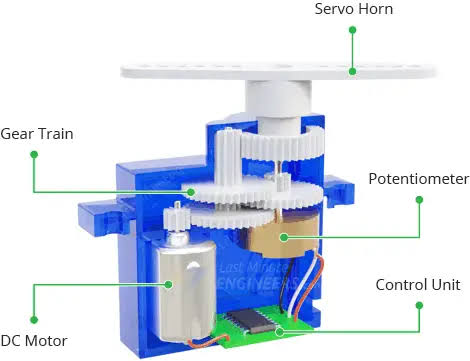
\includegraphics[width=0.55\textwidth]{images/sg90-internal.jpg}
	\caption{Struktur sirkuit kendali tertutup internal motor servo SG90.}
	\label{fig:sg90_karakteristik}
\end{figure}

\paragraph{Konsep dan Formulasi Matematis Terkait}
Hubungan antara lebar pulsa sinyal PWM ($W_{\text{pulsa}}$ dalam milidetik) dengan posisi sudut poros mekanis ($\theta$ dalam derajat) bersifat linier dan dirumuskan sebagai:

\begin{equation}
	\theta(W_{\text{pulsa}}) = \frac{W_{\text{pulsa}} - W_{\text{min}}}{W_{\text{maks}} - W_{\text{min}}} \times 180^\circ
	\label{eq:sg90_konversi_sudut}
\end{equation}

\noindent di mana:
\begin{itemize}
	\item $\theta$ = Posisi sudut target poros servo ($0^\circ \text{ s.d. } 180^\circ$).
	\item $W_{\text{pulsa}}$ = Lebar pulsa HIGH yang diberikan oleh mikrokontroler ($0{,}5 \text{ s.d. } 2{,}5\,\text{ms}$).
	\item $W_{\text{min}}$ = Lebar pulsa minimum untuk sudut $0^\circ$ ($\approx 0{,}5\,\text{ms}$).
	\item $W_{\text{maks}}$ = Lebar pulsa maksimum untuk sudut $180^\circ$ ($\approx 2{,}5\,\text{ms}$).
\end{itemize}

% ---------------------------------------------------------------------
\subsubsection{Alur Kerja Internal dan Protokol Komunikasi}
Alur operasi servo SG90 mengikuti pola \textbf{Input $\rightarrow$ Proses $\rightarrow$ Output}:
\begin{enumerate}
	\item \textbf{Input:} Penerimaan pulsa sinyal kendali PWM dari pin GPIO mikrokontroler secara berkala setiap periode $20\,\text{ms}$ ($50\,\text{Hz}$).
	\item \textbf{Proses:} IC internal mengevaluasi lebar pulsa masukan, mengukur posisi poros via potensiometer, dan menggerakkan motor DC hingga selisih posisi bernilai nol.
	\item \textbf{Output:} Pergerakan mekanis poros utama menuju sudut target dengan mempertahankan posisi tersebut menahan beban luar (\textit{holding torque}).
\end{enumerate}

\paragraph{Detail Sinyal Kontrol PWM dan Pewaktuan}
SG90 dikendalikan menggunakan protokol \textbf{Modulasi Lebar Pulsa} (\textit{Pulse Width Modulation} / PWM) dengan frekuensi standar $50\,\text{Hz}$ (periode total $T = 20\,\text{ms}$):
\begin{itemize}
	\item \textbf{Sinyal Periode ($T = 20\,\text{ms}$):} Sinyal PWM harus diulang terus-menerus setiap $20\,\text{ms}$ agar servo mempertahankan posisi sudutnya.
	\item \textbf{Sudut $0^\circ$ ($W_{\text{pulsa}} \approx 0{,}5\,\text{ms} / 500\,\mu\text{s}$):} Pulsa HIGH selama $0{,}5\,\text{ms}$ mengarahkan poros ke posisi sudut paling kiri ($0^\circ$).
	\item \textbf{Sudut $90^\circ$ ($W_{\text{pulsa}} \approx 1{,}5\,\text{ms} / 1500\,\mu\text{s}$):} Pulsa HIGH selama $1{,}5\,\text{ms}$ mengarahkan poros ke posisi tengah ($90^\circ$).
	\item \textbf{Sudut $180^\circ$ ($W_{\text{pulsa}} \approx 2{,}5\,\text{ms} / 2500\,\mu\text{s}$):} Pulsa HIGH selama $2{,}5\,\text{ms}$ mengarahkan poros ke posisi sudut paling kanan ($180^\circ$).
\end{itemize}

\begin{figure}[htbp]
	\centering
	\begin{tikzpicture}[x=0.22mm, y=10mm, >=Stealth, font=\sffamily\small]
		% Axis Utama
		\draw[->, color=gray!60, thick] (0, 0) -- (520, 0) node[right, color=black] {\textit{Waktu}};
		\draw[->, color=gray!60, thick] (0, 0) -- (0, 2.5) node[above, color=black] {Sinyal PWM};

		% Level Logika Y
		\node[left, font=\scriptsize] at (0, 1.8) {\textbf{HIGH (5V)}};
		\node[left, font=\scriptsize] at (0, 0.4) {\textbf{LOW (0V)}};
		\draw[dotted, color=gray!40] (0, 1.8) -- (500, 1.8);
		\draw[dotted, color=gray!40] (0, 0.4) -- (500, 0.4);

		% Gelombang Pulsa 1 (Sudut 0 Derajat)
		\draw[ultra thick, color={rgb,255:red,30;green,64;blue,175}]
		(0, 0.4) -- (20, 0.4) -- (20, 1.8) -- (45, 1.8) -- (45, 0.4) -- (180, 0.4);

		% Gelombang Pulsa 2 (Sudut 90 Derajat)
		\draw[ultra thick, color={rgb,255:red,15;green,118;blue,110}]
		(180, 0.4) -- (180, 1.8) -- (255, 1.8) -- (255, 0.4) -- (340, 0.4);

		% Gelombang Pulsa 3 (Sudut 180 Derajat)
		\draw[ultra thick, color={rgb,255:red,217;green,119;blue,6}]
		(340, 0.4) -- (340, 1.8) -- (465, 1.8) -- (465, 0.4) -- (500, 0.4);

		% Garis Bantu Vertikal Periode
		\draw[dashed, color=gray!50] (20, 2.3) -- (20, 0.2);
		\draw[dashed, color=gray!50] (180, 2.3) -- (180, 0.2);

		% Anotasi Lebar Pulsa
		\draw[stealth-stealth, color={rgb,255:red,30;green,64;blue,175}, thick] (20, 2.0) -- (45, 2.0)
		node[midway, above, font=\tiny] {\shortstack{$0{,}5\,\text{ms}$\\($0^\circ$)}};
		\draw[stealth-stealth, color={rgb,255:red,15;green,118;blue,110}, thick] (180, 2.0) -- (255, 2.0)
		node[midway, above, font=\tiny] {\shortstack{$1{,}5\,\text{ms}$\\($90^\circ$)}};
		\draw[stealth-stealth, color={rgb,255:red,217;green,119;blue,6}, thick] (340, 2.0) -- (465, 2.0)
		node[midway, above, font=\tiny] {\shortstack{$2{,}5\,\text{ms}$\\($180^\circ$)}};

		% Anotasi Periode Total 20ms
		\draw[stealth-stealth, color=black, thick] (20, -0.4) -- (180, -0.4)
		node[midway, below, font=\tiny] {Periode Total $T = 20\,\text{ms}$ ($50\,\text{Hz}$)};
	\end{tikzpicture}
	\caption{Diagram pewaktu sinyal kontrol PWM dan durasi pulsa pemicu sudut posisi servo SG90.}
	\label{fig:sg90_timing}
\end{figure}

Pengaturan pulsa ini pada mikrokontroler umumnya ditangani langsung melalui pustaka standar seperti \texttt{Servo.h} pada ekosistem Arduino, sehingga pengguna cukup menentukan nilai sudut target ($0\text{ s.d. }180^\circ$) pada tingkatan aplikasi.

% ---------------------------------------------------------------------
\subsubsection{Besaran yang Diukur atau Dikendalikan}
SG90 bertindak sebagai pengatur posisi sudut mekanis. Parameter batas operasional kendali posisi servo dirangkum pada Tabel~\ref{tab:sg90_karakteristik_besaran}.

\begin{table}[H]
	\centering
	\caption{Karakteristik besaran operasional SG90 Mikro Servo}
	\label{tab:sg90_karakteristik_besaran}
	\small
	\begin{tabularx}{\textwidth}{@{} p{3.8cm} >{\hsize=0.7\hsize}X >{\hsize=1.3\hsize}X @{}}
		\toprule
		Parameter                                  & Nilai                                                     & Keterangan                                                \\
		\midrule
		Besaran Utama                              & Posisi Sudut Mekanis ($\theta$)                           & Sudut rotasi poros luaran                                 \\
		Rentang Kerja Sudut                        & $0^\circ \text{ s.d. } 180^\circ$                           & Rentang pergerakan rotasi maksimum                        \\
		Torsi Tahan (\textit{Stall Torque})        & $1{,}8\,\text{kg}\cdot\text{cm}$ (pada $4{,}8\,\text{V}$) & Kemampuan menahan beban maksimum sebelum poros tertahan   \\
		Kecepatan Operasional                      & $0{,}12\,\text{s}/60^\circ$ (pada $4{,}8\,\text{V}$)      & Kecepatan rotasi poros tanpa beban                        \\
		Lebar Pita Mati (\textit{Dead Band Width}) & $7\,\mu\text{s}$                                          & Toleransi batas minimum perubahan pulsa pemicu pergerakan \\
		Presisi Posisi                             & $\approx 1^\circ \text{ s.d. } 2^\circ$                     & Akurasi penempatan posisi sudut mekanis                   \\
		\bottomrule
	\end{tabularx}
\end{table}

% ---------------------------------------------------------------------
\subsubsection{Karakteristik Sinyal}
Karakteristik sinyal elektrik antarmuka kontrol SG90 dirangkum pada Tabel~\ref{tab:sg90_sinyal}.

\begin{table}[H]
	\centering
	\caption{Karakteristik sinyal kontrol PWM SG90 Mikro Servo}
	\label{tab:sg90_sinyal}
	\small
	\begin{tabularx}{\textwidth}{@{} p{3.8cm} >{\hsize=0.8\hsize}X >{\hsize=1.2\hsize}X @{}}
		\toprule
		Aspek                   & Nilai                                                                      & Keterangan                                                \\
		\midrule
		Jenis Sinyal            & Pulsa PWM Analog/Digital                                                   & Lebar pulsa menentukan posisi sudut                       \\
		Level Logika Sinyal     & $3{,}3\text{ s.d. }5{,}0\,\text{V}$ (TTL)                                    & Kompatibel langsung dengan GPIO MCU                       \\
		Frekuensi Sinyal PWM    & $50\,\text{Hz}$ (Periode $20\,\text{ms}$)                                  & Standar frekuensi \textit{update} kontrol servo           \\
		Rentang Lebar Pulsa     & $0{,}5 \text{ s.d. } 2{,}5\,\text{ms}$ ($500 \text{ s.d. } 2500\,\mu\text{s}$) & Representasi posisi sudut $0^\circ \text{ s.d. } 180^\circ$ \\
		Arus Pin Sinyal Kontrol & $< 1\,\text{mA}$                                                           & Sangat kecil, aman dikendalikan langsung oleh GPIO MCU    \\
		\bottomrule
	\end{tabularx}
\end{table}

% ---------------------------------------------------------------------
\subsubsection{Pin, Catu Daya, dan Antarmuka}
Motor servo SG90 dilengkapi kabel 3-jalur terintegrasi yang terhubung ke \textit{connector header} 3-pin standar ($2{,}54\,\text{mm}$ \textit{pitch}).

\begin{figure}[H]
	\centering
	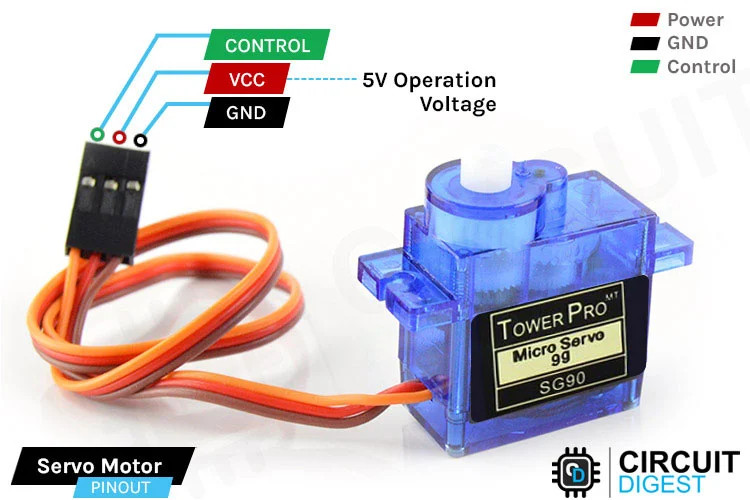
\includegraphics[width=0.5\textwidth]{images/sg90-pinout.jpg}
	\caption{Pemetaan pin dan antarmuka modul mikro servo SG90.}
	\label{fig:sg90_pinout}
\end{figure}

\begin{table}[H]
	\centering
	\caption{Pemetaan pin dan fungsi kabel SG90 Mikro Servo}
	\label{tab:sg90_pin}
	\small
	\begin{tabularx}{\textwidth}{@{} p{3.2cm} p{2.2cm} X @{}}
		\toprule
		Pin Antarmuka & Fungsi         & Keterangan                                                     \\
		\midrule
		VCC           & $V_{CC}$       & Catu daya positif motor ($4{,}8\text{ s.d. }6{,}0\,\text{V DC}$) \\
		GND           & GND            & Referensi ground bersama ($0\,\text{V}$)                       \\
		Control       & Sinyal Kontrol & Jalur masukan pulsa PWM dari pin GPIO mikrokontroler           \\
		\bottomrule
	\end{tabularx}
\end{table}

\subsubsection{Kebutuhan Catu Daya}
SG90 beroperasi optimal pada tegangan $4{,}8\text{ s.d. }6{,}0\,\text{V DC}$. Konsumsi arus servo bervariasi secara signifikan tergantung pada kondisi beban mekanis:
\begin{itemize}
	\item Arus kondisi siaga (\textit{idle current}): $\approx 10\text{ s.d. }20\,\text{mA}$.
	\item Arus saat bergerak tanpa beban (\textit{running current}): $\approx 100\text{ s.d. }250\,\text{mA}$.
	\item Arus beban puncak / macet (\textit{stall current}): $\approx 500\text{ s.d. }650\,\text{mA}$.
\end{itemize}

Karena arus macet (\textit{stall current}) dapat mencapai $\approx 650\,\text{mA}$, pasokan daya sangat disarankan dihubungkan ke sumber daya $5\,\text{V}$ eksternal atau bus daya utama MCU yang memadai, serta menyatukan seluruh jalur \textit{ground} (\textit{common ground}).

% ---------------------------------------------------------------------
\subsubsection{Spesifikasi Penting dari Datasheet}
Parameter teknis operasional penting yang diambil dari \textit{datasheet} resmi TowerPro dirangkum pada Tabel~\ref{tab:sg90_spesifikasi}.

\begin{table}[H]
	\centering
	\caption{Spesifikasi teknis penting SG90 Mikro Servo}
	\label{tab:sg90_spesifikasi}
	\small
	\begin{tabularx}{\textwidth}{@{} X c @{}}
		\toprule
		Parameter                                                  & Nilai                                            \\
		\midrule
		Tegangan Kerja Operasional ($V_{CC}$)                      & $4{,}8 \text{ s.d. } 6{,}0$ $\text{V DC}$          \\
		Torsi Tahan (\textit{Stall Torque} pada $4{,}8\,\text{V}$) & $1{,}8$ $\text{kg}\cdot\text{cm}$                \\
		Kecepatan Operasional (pada $4{,}8\,\text{V}$)             & $0{,}12$ $\text{s} / 60^\circ$                   \\
		Lebar Pita Mati (\textit{Dead Band Width})                 & $7$ $\mu\text{s}$                                \\
		Sudut Rotasi Maksimum                                      & $180$ $\text{derajat } (^\circ)$                 \\
		Berat Komponen                                             & $\approx 9$ $\text{gram}$                        \\
		Dimensi Fisik ($L \times W \times H$)                      & $22{,}8 \times 12{,}2 \times 28{,}5$ $\text{mm}$ \\
		Suhu Operasional Lingkungan                                & $0 \text{ s.d. } +55$ $^\circ\text{C}$             \\
		\bottomrule
	\end{tabularx}
\end{table}

% ---------------------------------------------------------------------
\subsubsection{Koneksi dengan Mikrokontroler dan Implementasi Kode}
Motor servo SG90 dihubungkan ke mikrokontroler Arduino Mega 2560 untuk mengendalikan pergerakan posisi sudut mekanis secara tepat. Periferal internal mikrokontroler yang dialokasikan mencakup satu pin \textbf{GPIO Digital PWM} (digerakkan oleh \textit{Hardware Timer/Counter} ATmega2560) guna membangkitkan sinyal pulsa kontrol berfrekuensi $50\,\text{Hz}$ secara kontinu.

\paragraph{Rangkaian Skematik dan Simulasi}
Pengujian antarmuka perangkat keras divalidasi melalui platform simulasi Wokwi dengan pemetaan koneksi sebagai berikut:
\begin{itemize}
	\item \textbf{Koneksi Catu Daya:} Kabel daya positif (merah) dihubungkan ke bus daya $5\,\text{V DC}$ Arduino Mega 2560, dan kabel ground (cokelat/hitam) dihubungkan ke saluran ground bersama (\textit{common ground}).
	\item \textbf{Koneksi Sinyal Kontrol:} Kabel sinyal PWM (oranye/kuning) dihubungkan langsung ke pin digital 9 Arduino Mega 2560 yang mendukung fitur modulasi lebar pulsa berbasis \textit{hardware timer}.
\end{itemize}

\begin{figure}[htbp]
	\centering
	% Gambar skematik / visualisasi simulasi SG90 Mikro Servo pada Wokwi
	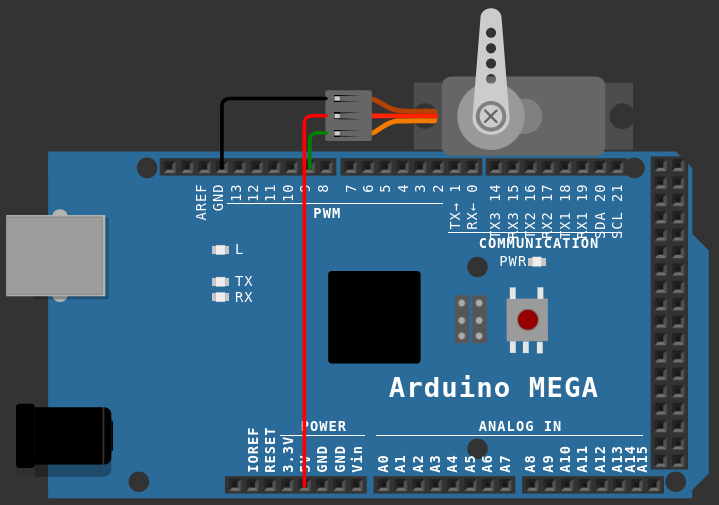
\includegraphics[width=0.45\textwidth]{images/servo_wokwi.png}
	\caption{Rangkaian simulasi pengujian servo pada platform Wokwi.}
	\label{fig:sg90_module_image}
\end{figure}

Rincian pemetaan koneksi fisik antara pin kabel SG90 mikro servo dan fungsi periferal mikrokontroler ATmega2560 dirangkum pada Tabel~\ref{tab:sg90_mcu_mapping}.

\begin{table}[H]
	\centering
	\caption{Pemetaan antarmuka SG90 mikro servo ke Arduino Mega 2560}
	\label{tab:sg90_mcu_mapping}
	\small
	\begin{tabularx}{\textwidth}{@{} p{3.5cm} p{3.8cm} X @{}}
		\toprule
		Kebutuhan Komponen      & Fitur MCU                         & Alasan Pemilihan \& Fungsi                                                                                             \\
		\midrule
		Sinyal Kontrol PWM      & Pin GPIO PWM Digital 9            & Membangkitkan pulsa sinyal $50\,\text{Hz}$ dengan lebar pulsa $0{,}5\text{ s.d. }2{,}5\,\text{ms}$ untuk penentuan sudut \\
		Pewaktuan Pulsa Presisi & \textit{Hardware Timer} MCU       & Menjaga konsistensi durasi pulsa PWM tanpa terganggu oleh proses pemrosesan utama                                      \\
		Catu Daya Motor DC      & Bus Daya $5\,\text{V}$ \& GND MCU & Menyediakan tegangan kerja $5\,\text{V DC}$ dan konsumsi arus operasional motor servo                                  \\
		\bottomrule
	\end{tabularx}
\end{table}

\paragraph{Kode Demo Pengujian}
Berikut adalah implementasi kode program C++ berbasis pustaka \texttt{Servo.h} untuk menguji pergerakan sweep posisi sudut servo SG90 secara bertahap pada Arduino Mega 2560:

\begin{lstlisting}[language=C++, caption={Kode program pengujian pergerakan posisi sudut SG90 mikro servo pada Arduino Mega 2560}, label={lst:sg90_code}]
#include <Servo.h>
#define SERVO_PIN 9

Servo myServo;

void setup() {
  Serial.begin(9600);
  Serial.println(F("Inisialisasi Pengujian SG90 Mikro Servo..."));

  myServo.attach(SERVO_PIN);
  myServo.write(0);
  delay(1000);
}

void loop() {
  Serial.println(F("[POSISI] Memutar ke sudut 0 Derajat"));
  myServo.write(0);
  delay(2000);

  Serial.println(F("[POSISI] Memutar ke sudut 90 Derajat"));
  myServo.write(90);
  delay(2000);

  Serial.println(F("[POSISI] Memutar ke sudut 180 Derajat"));
  myServo.write(180);
  delay(2000);

  Serial.println(F("[SWEEP] Melakukan pergerakan bertahap (0 -> 180 Derajat)"));
  for (int pos = 0; pos <= 180; pos += 10) {
    myServo.write(pos);
    delay(100);
  }

  Serial.println(F("[SWEEP] Melakukan pergerakan bertahap (180 -> 0 Derajat)"));
  for (int pos = 180; pos >= 0; pos -= 10) {
    myServo.write(pos);
    delay(100);
  }
}
\end{lstlisting}

\paragraph{Gambaran Hasil Pembacaan}
Tampilan log keluaran pada \textit{Serial Monitor} saat simulasi pengujian pergerakan sudut servo SG90 dijalankan adalah sebagai berikut:

\begin{verbatim}
Inisialisasi Pengujian SG90 Mikro Servo...
[POSISI] Memutar ke sudut 0 Derajat
[POSISI] Memutar ke sudut 90 Derajat
[POSISI] Memutar ke sudut 180 Derajat
[SWEEP] Melakukan pergerakan bertahap (0 -> 180 Derajat)
[SWEEP] Melakukan pergerakan bertahap (180 -> 0 Derajat)
\end{verbatim}
